% Modèle pour article soumis à SGE 2014
% http://sge2014.sciencesconf.org/
%
% Auteur : Romain Corcolle, LGEP (Laboratoire de Génie Electrique de Paris)
% modifié par : Pierre Haessig et Thibaut Kovaltchouk, SATIE
% Licence : document placé dans le domaine public (CC0)
%
% Pour récupérer la dernière version du template :
% https://github.com/pierre-haessig/template-SGE2014
% Pour rapporter un problème :
% https://github.com/pierre-haessig/template-SGE2014/issues
\documentclass[a4paper,10pt,twocolumn]{article}

\usepackage[utf8x]{inputenc}
\usepackage[french]{babel}
\usepackage{graphicx,times}
\usepackage[T1]{fontenc}
\usepackage{amsmath}
\usepackage[font=footnotesize]{caption}
\usepackage{fancyhdr}
\usepackage[explicit]{titlesec}
\usepackage{hyperref}
\usepackage[square,comma,numbers]{natbib}
\usepackage{tabularx}

\newcolumntype{L}[1]{>{\raggedright\arraybackslash}p{#1}}
\newcolumntype{C}[1]{>{\centering\arraybackslash}p{#1}}
\newcolumntype{R}[1]{>{\raggedleft\arraybackslash}p{#1}}


\renewcommand{\bibsection}{}
\def\bibfont{\footnotesize}
\setlength{\bibsep}{0.2em}
\setlength{\bibhang}{10em}

\hypersetup{colorlinks=true, urlcolor=blue, citecolor=black, linkcolor = black}

\addto\captionsfrench{\def\figurename{Fig.}}
\addto\captionsfrench{\def\tablename{Tableau}}

\captionsetup[figure]{labelsep=period, justification=raggedright, singlelinecheck=false}
\captionsetup[table]{labelsep=period, justification=centering, singlelinecheck=false}

% extra line spacing:
\usepackage{setspace}
\setstretch{1.15}

\parindent 10pt

\setlength{\voffset}{-0.55in}
\setlength{\topmargin}{0cm}

\setlength{\headsep}{-0.10cm}
\setlength{\topskip}{0.7cm}

\setlength{\hoffset}{-1in}
\setlength{\oddsidemargin}{1.3cm}
\setlength{\evensidemargin}{1.3cm}

\setlength{\textheight}{25.5cm}
\setlength{\textwidth}{18.5cm}

\setlength{\columnsep}{0.64cm}

\titleformat{\section}
  {\scshape}{\thesection.}{0.5em}{#1}
\titleformat{\subsection}
  {\itshape}{\thesubsection.}{1.5em}{#1}
\titleformat{\subsubsection}
  {\itshape}{\thesubsubsection.}{1.5em}{#1}
  
\setlength{\parskip}{0.3em plus0.05em minus0.02em}
\titlespacing\section{0pt}{0.3em}{0em}
\titlespacing\subsection{0pt}{0.3em}{0em}
\titlespacing\subsubsection{0pt}{0.3em}{0em}

\fancyhf{}
\fancyhead[R]{\fontsize{8pt}{8pt}\selectfont \textsc{Symposium de Génie Électrique (SGE’14) : EF-EPF-MGE 2014, 8--10 juillet 2014, ENS Cachan, France}}
\renewcommand{\headrulewidth}{0pt}

\pagestyle{empty}

\title{
\fontsize{24pt}{24pt}\selectfont
Titre de la communication (Style ‘Titre’)
}

\author{
\fontsize{11pt}{11pt}\selectfont
Prénom NOM des auteurs (Style ‘Nom’)\\
\fontsize{10pt}{10pt}\selectfont
Affiliation des auteurs (Style ‘Affiliation’)
}

\date{}


\begin{document}

\maketitle
\thispagestyle{fancy}


\fontsize{9pt}{9pt}\selectfont
\textbf{RÉSUMÉ -- Écrire un résumé de la communication de 15 lignes maximum. Ce résumé doit présenter de façon synthétique les objectifs du travail présenté, les principaux résultats et insister sur les originalités du travail. (Style ‘Résumé’)}\\

\textbf{\textit{Mots-clés -- Écrire ici une liste n’excédant pas 8 mots-clés significatifs. (Style ‘Mots-Clés’).}}

\fontsize{10pt}{10pt}\selectfont


\section{Introduction  (Style ‘Titre 1’)}

Décrire le contexte et les objectifs du travail. Positionner le travail par rapport à la littérature et aux principaux travaux antérieurs. Présenter le plan de la communication. (Style ‘Normal’).

\section{Titre de section (Style ‘Titre 1’)}

Développer dans les sections, sous-sections et sous sous-sections (ne pas excéder 3 niveaux hiérarchiques) les travaux réalisés en présentant les grandes étapes et les principaux résultats.

\textbf{L’article final de la communication doit comporter au maximum 10 pages et doit respecter le format décrit dans ce document. La taille du fichier pdf est par ailleurs limitée à 3,5~Mo.}

\subsection{Titre de sous-section (Style ‘Titre 2’)}

Les tableaux, figures et équations doivent respecter les numérotations et formats ci-après. Les figures (Style ‘Images’) et tableaux (Style ‘Tableaux’) doivent être centrés et légendées. Les équations (Style ‘Equation’, 10 pts, centré) seront centrées et numérotées (style ‘Numéro d’équation’, Times New Roman, 10 pts, aligné à droite) et une ligne pourra être laissée libre avant et après chaque équation.

\begin{figure}[!ht]
	\begin{center}
		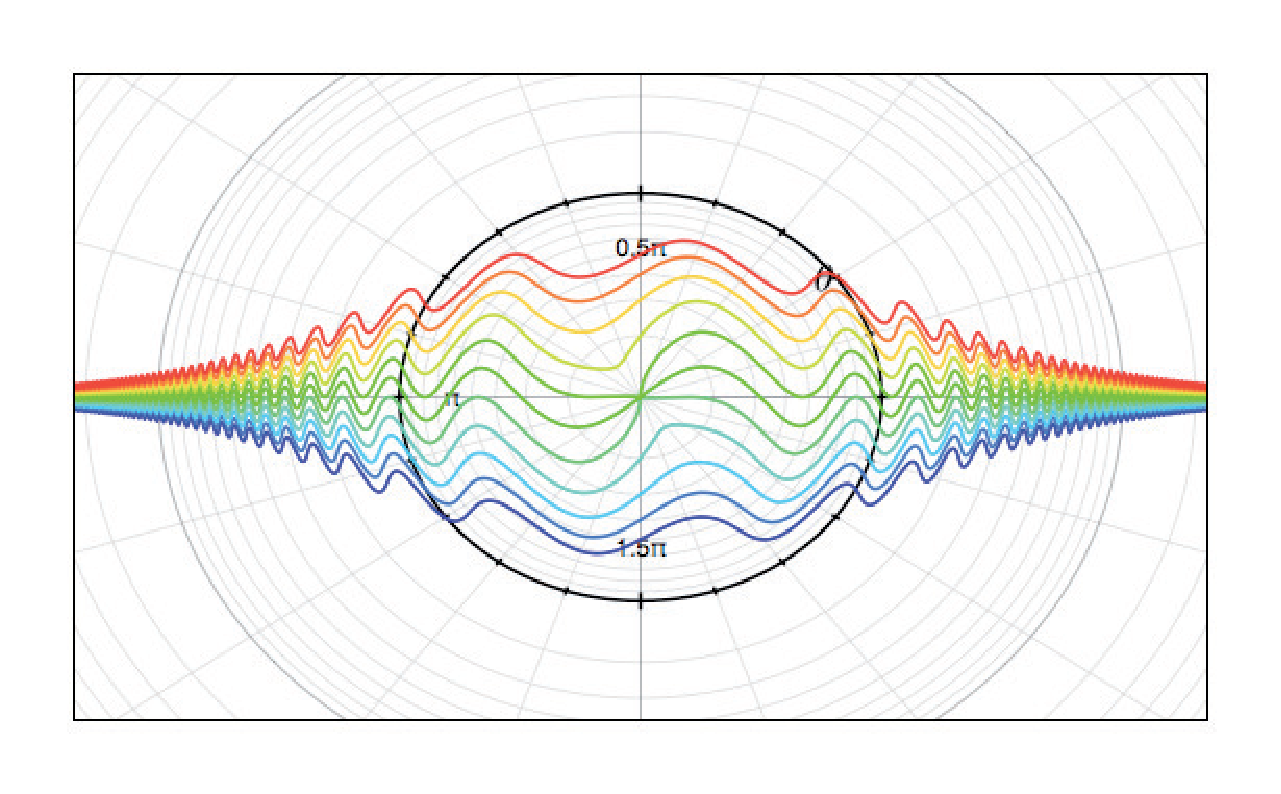
\includegraphics[width=0.9\columnwidth]{fig_1.pdf}
	\end{center}
	
	\caption{Mettre ici le titre de la figure}
	\label{fig_1}
\end{figure}

\begin{table}[!h]
	\caption{Mettre ici le titre du tableau}
	
\centering
		\begin{tabular}{|>{\footnotesize}L{1.4cm}|>{\footnotesize}L{1.5cm}|>{\footnotesize}L{2.4cm}|>{\footnotesize}L{2.1cm}|}
			\hline
			\textbf{Titre colonne 1} & \textbf{Titre colonne 2} & \textbf{Style (‘Titre colonnes tableaux’)} & \textbf{} \\
			\hline
			Donnée 1 & Style (Cellules tableaux’) & & \\
			\hline
			Donnée 2 & & & \\
			\hline
		\end{tabular}

	
	\label{tab_1}
\end{table}

\subsubsection{Titre de sous sous-section (Style ‘Titre 3’)}

\begin{equation}
	y = f(x) + \sum_{k=1}^{\infty} h_k \cdot sin(k \omega t)
	\label{eq_1}
\end{equation}

\section{Soumission de la communication}

La soumission se fait en ligne à partir du site électronique de la conférence : \url{http://sge2014.sciencesconf.org/} (voir la rubrique ‘Soumission en ligne des communications’).

Le fichier soumis sera préalablement converti au format PDF avec les polices incorporées et ne devra pas excéder la taille maximale de 3.5 Mo.

\section{Conclusions}

Rappeler les principaux résultats marquants et originaux du travail. Le cas échéant, proposer des perspectives au travail présenté.

\section{Remerciements}

Cette partie (facultative) doit être placée entre la conclusion et les références.

\section{Références}

Citer ici les principales références du travail réalisé (style ‘Références’). Privilégier les références les plus pertinentes et les publications originelles. Numéroter les références de la même façon que dans l’exemple ci-dessous – par ordre d’apparition dans le texte. Exemple XX\cite{bib_1} et YY\cite{bib_2,bib_3}.

\begin{thebibliography}{1}


\bibitem{bib_1}{Marianne LOSSEC, Bernard MULTON, Hamid BEN AHMED, « Etude d'un générateur micro-cinétique : modélisation énergétique et optimisation du transfert d'énergie », Électrotechnique du Futur 2009, Compiègne (France).}

\bibitem{bib_2}{Denis LABROUSSE, Bertrand Revol, Fabien ADAM, François COSTA, Bruno PLIQUET, « Modélisation et simulation par fonctions de couplage d’une structure de puissance », Electronique de Puissance du Futur 2008, Tours (France).}

\bibitem{bib_3}{T.T. Nguyen, L. Daniel, F. Bouillault, X. Mininger, « Modélisation d’un capteur magnétoélectrique par la méthode des éléments finis », MGE, 2010, Montpellier (France).}


\end{thebibliography}


\end{document}


